\chapter{Evaluation}
\label{ch:evaluation}
% terminology: attentional data = 'focus rate'

\section{Introduction} % (fold)
\label{sec:evaluation_introduction}

This chapter reports on a number of experiments on the wePorter system. We report on the feedback that is received from users' interaction through the use of the wePorter web interface. We show how this data can be used for the purposes of filtering segments within a video and the reconfiguration of these segments into a new video story. We present results from a user evaluation study on the merit of filtered and reconfigured content and also include results obtained from a user questionnaire supplied along with our main experiment.

% section introduction (end)

\section{Preliminary Experiments}
\label{sec:preliminary_experiments}

\subsection{Positional Bias}
Positioning two video's one on top of the other, might inflict a bias for users in their attentional behaviour. It might be the case that videos on the top are systematically more attended to than videos displayed below. We've experimented to see whether such positioning bias effects occur.

To see whether the positioning of a video has effect on users' attentional behaviour, we've presented two groups of users the same two videos playing in parallel and varied their relative positioning. In two trials, participants were divided by random into control group and test group. The first trial was conducted with 37 participants (24 control, 13 test), the second with 32 (18 control, 14 test). In each trial, test group participants were show the same two videos as the control group, but their positioning was flipped. Figure \ref{fig:exp_posbias} shows a visual explanation of the experimental setup.

\begin{figure}[htbp]
  \centering
    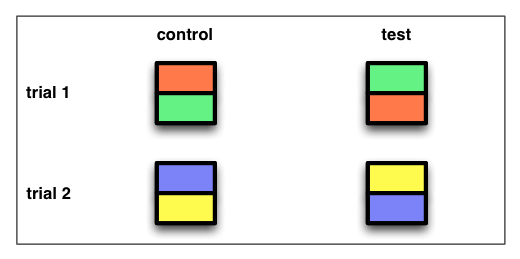
\includegraphics[width = .5\textwidth]{img/exp_posbias}
  \caption{Setup for Positional Bias Experiment}
  \label{fig:exp_posbias}
\end{figure}


\subsection{Context Dependency}
We propose a statistical analysis of interaction data to inform the reconfiguration of initially unstructured video parts. We hypothesise that:
\begin{enumerate}
  % \item The perceived quality of a video reconfiguration is dependent on the sequential ordering of its internal parts
  \item Users' attentional behaviour depends on the sequential ordering of video parts
  \item Data about users' attentional behaviour can indicate what are preferred orderings.
\end{enumerate}

Before we investigate the second hypothesis in section \ref{sec:main_experiments}, we must scrutinise the first. In order to test whether users' attentional behaviour is dependent on the sequential ordering of video parts we have run a experiment in two trials. The first of these had 35 participants, the second 28. In each trial participants were presented with with a two sequences of three video parts playing back continuously using the parallel video player described in section \ref{sec:weporter_interface}. Based on random picks, roughly half of the participants were labelled as control group the others as test group. Participants in this group where shown two sequences where all video parts originated from different sources. This was changed for the second group, where participant were shown parts across the sequences that clearly belong to the same source video. 

The first trial presented test group users with a first part in the bottom sequence that was followed by a part from the same source video as the third part in the top video. The second trial presented test group users with pieces from the same source video in the first and third part of the top sequence and second part of the bottom sequence. The baseline sequences shown to control group participants had video parts of different sources on all positions and had final parts of both sequences identical to test group users. A visual description of these conditions is shown in figure \ref{fig:exp_context}. Where we use the same conventions to display sequences, video parts and colouring to indicate source videos as in figure \ref{fig:framework}.

\begin{figure}[htbp]
  \centering
    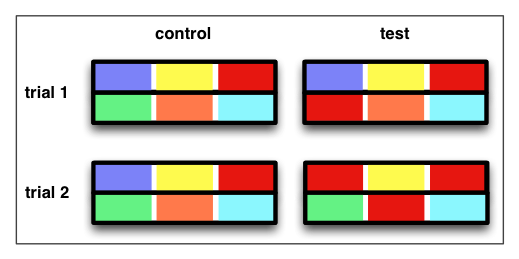
\includegraphics[width = .5\textwidth]{img/exp_context}
  \caption{Setup for Context Dependency Experiment}
  \label{fig:exp_context}
\end{figure}


The effects of Positional Bias and Context Dependency are mainly interesting when experiments involve large amounts of data. This is first of all because of the increased statistical power that large data set bring to the table for these experiments themselves. Second, the experiments, in particular the one studying influences of context, are aimed at acquisition of knowledge that helps to steer the design of methods that needs many more data points that the limited set we have been able to acquire in our main experiment. Initial sets of data for both the Positional Bias and Context Dependency experiment have been obtained, but as they do little for the purpose of the current thesis, their analyses is left out of this work. The descriptions of the two experiments are included to indicate the two issues at hand and point to possible ways to investigate.

\section{Main Experiments} % (fold)
\label{sec:main_experiments}

Our main experiments use the system framework described in section \ref{sec:weporter_implementation} for the preparation and presentation of video content, data capture from user interaction and storage of interaction data. The experiments we report on here are based on the interactions from a total of 51 persons who all participated once over a period of a week.

\subsection{Setup}
For our main experiments we use a set of 10 unedited, user-generated videos returned in response to the query ``Diamond Jubilee London'' on YouTube. The videos along with their title, length and view count at time of retrieval is shown in table \ref{videos}. As mentioned in section \ref{sec:weporter_implementation}, we divide source videos into video parts of equal length and generate two sequences consisting of an equal number of video parts to present in parallel. Partitioning the source videos from table \ref{videos} yields 142 separate video parts.

\begin{table}
   \begin{tabular}{ | l | l | p{8cm} | p{1.3cm} | l |}
     \hline
     \textbf{Id} & \textbf{File Name}	          & \textbf{Title}	  & \textbf{Length (sec)} & \textbf{Views} \\ \hline
     1	 & ``jubilee\_01.webm''	& ``Diamond Jubilee London 5th June 2012 The Mall Video 3'' & 186                             & 45   \\ \hline
     2	 & ``jubilee\_02.webm''	& ``Diamond jubilee London 5th June 2012 The Mall'' & 47                                      & 108  \\ \hline
     3	 & ``jubilee\_03.webm''	& ``London Thames - Queens Diamond Jubilee Pageant - Dunkirk Little Ships, June 2012'' & 234  & 2304\\ \hline
     4	 & ``jubilee\_04.webm''	& ``My Diamond Jubilee video!'' & 54                                                          & 28   \\ \hline
     5	 & ``jubilee\_05.webm''	& ``Queens Barge. Diamond Jubilee London 2012 VIDEO Ursula Maxwell-Lewis 0053'' & 163         & 88   \\ \hline
     6	 & ``jubilee\_06.webm''	& ``Queens diamond jubilee London 5th June 2012'' & 30                                        & 43   \\ \hline
     7	 & ``jubilee\_07.webm''	& ``Queens Diamond Jubilee Procession, 5th June 2012, London, UK'' & 133                      & 58   \\ \hline
     8	 & ``jubilee\_08.webm''	& ``Queens Elizabeth 60th Diamond Jubilee London 2012. 1st'' & 73                             & 203  \\ \hline
     9	 & ``jubilee\_09.webm''	& ``Queens Elizabeth 60th Diamond Jubilee London 2012. 2nd'' & 165                            & 246  \\ \hline
     10 & ``jubilee\_11.webm''	& ``Queens Elizabeth 60th Diamond Jubilee London 2012. 14th'' & 390                           & 88   \\ \hline
   \end{tabular}
   \caption{Source Videos used for the main experiments (Views count accessed on 23-09-2012)}
   \label{videos}
\end{table}

The sequence loading procedure shown in algorithm \ref{alg:genseqs}, prepares two parallel sequences consisting of six video parts each. Each interaction thus presents a user with twelve video parts. For the 51 interactions focus rates are captured. Video parts have each been presented between 3 and 7 times. 

\subsection{Parallel Play Interaction Data} % (fold)
\label{sub:parallel_play_interaction_data}

\subsubsection{Clean Data} % (fold)

Data returned from the capturing of attentional behaviour in the parallel player interface might have several deficiencies that we deal with by preprocessing the data before we start analysis. Deficiencies range from artefacts induced by the inaccurate functioning of the interface to users' behaviour patterns that make their data less revealing. Such patterns are expected to be caused by misunderstood instructions and minor technical shortcomings in the implementation of the web interface.

Some entries show focus rates of both sequences consistently valued at zero. This can either be caused by a malfunction of the focus counter functionality or by a user simply not focussing on either of the videos. These entries are completely deleted from the dataset. Although not present in the data required in our current experiments, focus rates of segments within a single sequence might also be consistently high valued. This indicates behaviour of someone who decided not to change focus. Although it might be a sign that the user is simply most interested in the one particular sequence, we would also discard these entries as they are most likely to result of a lazy participant who decided not to move the mouse or someone who misunderstood the instructions. Moreover, interactions patterns that aren't the cause of active exploration of the content are not likely to reveal useful information with regard to a user's interest.

The unit of measurement for focus time as captured by the parallel play interface is 100ms. A ten second clip can theoretically thus acquire a focus rate of 100, indicating a user has focussed for the complete duration of 10-seconds. A user dividing focus over two parallel videos would result in two focus rate around 50 that together add up to maximally 100. Practically however, many focus pairs in the dataset have a combined sum over 100. This is most likely cause by the method of logging focus counts. Although counters are only increased when a video is playing to prevent a video's potential load time to contribute to its focus rate, there may still be glitches induces by videos not playing bad continuously in the web browser. Also, moving the mouse quickly back and forth between the two videos can cause the two counters to be increased during a single time frame of 100 ms. These technical shortcomings should be addressed in a future implementation. 

Because of the varying sum of focus rate pairs, it is more indicative to look at the ratio between the two parallel rates than to absolute rates. This way a focus rate of 50 in pair $\{focus(50,u_j), focus(50,u_j)\}$ has a different contribution than in pair $\{focus(50,u_k), focus(0,u_k)\}$. Likewise, it ensures that a rate of 30 in the pair $\{focus(30,u_l), focus(30,u_l)\}$ has a contribution equal to that of the rate of 50 in the pair received from user $u_j$. 

\begin{figure}[htbp]
  \centering
    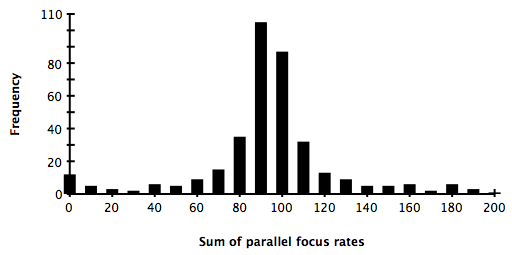
\includegraphics[width = .6\textwidth]{img/histogram_ratingsSum}
  \caption{Occurrence of different sums of parallel focus rates}
  \label{fig:histogram_ratingsSum}
\end{figure}

A further processing step is to weigh the ratios depending on the size of their sum. This is to emphasise focus pairs with a sum around 100 as this indicates a user has spend the full playing time focussing on at least on of the presented sequences. figure \ref{fig:histogram_ratingsSum} shows the distribution of the sum of parallel focus counts. Focus pairs whose rates sum to values between 20 and 160 are weighted once, sums between 70 and 120 are weighted twice. Focus rates that sum to other values are discarded.

Figure \ref{fig:videoparts_focus} shows both average absolute focus rates and average weighted ratios received for all video parts. For clarity, ratios in the plot are scaled by a factor 100 to match the absolute rates' order of magnitude.

\begin{figure}[htbp]
  \centering
    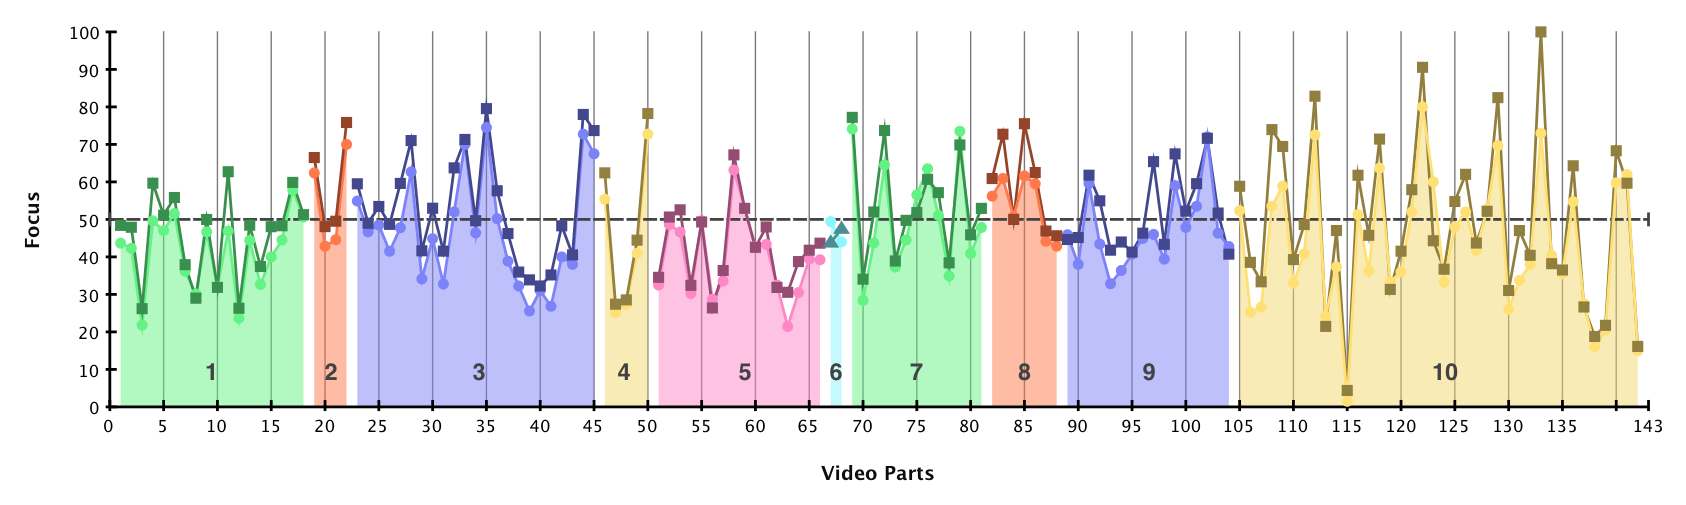
\includegraphics[width=\textwidth]{img/videoparts_focus}
  \caption{Average focus rates and weighted focus ratios for individual video parts}
  \label{fig:videoparts_focus}
\end{figure}

% subsection parallel_play_interaction_data (end)

\subsection{Attention-based filtering} % (fold)
\label{sub:attention_based_filtering}

Considering the assumption that user interest may be inferred from many users' focus data across different interactions, we can look at the focus data and use it to form a selections of \emph{best} and \emph{worst} attended-to video parts.

To find a reasonable amount of video parts for most of the source videos in the experiment that make it into the \emph{best} and \emph{worst} sets, we consider focus ratings over 60 and below 40 respectively. Selection of parts for filtering out can be straight forward based on a ranking of all video parts within the \emph{worst} set of parts and a rejection of the $x\%$ video parts with the lowest rates. For an optimal selection for reconfiguration, a slightly more complex procedure may be preferred, as simply selecting the top $y\%$ of the \emph{best} set may result in several video parts from the same source video. This may not be desired for reconfiguration and in that case diversity in source videos should be promoted in the selection procedure.

\begin{figure}[htbp]
  \centering
    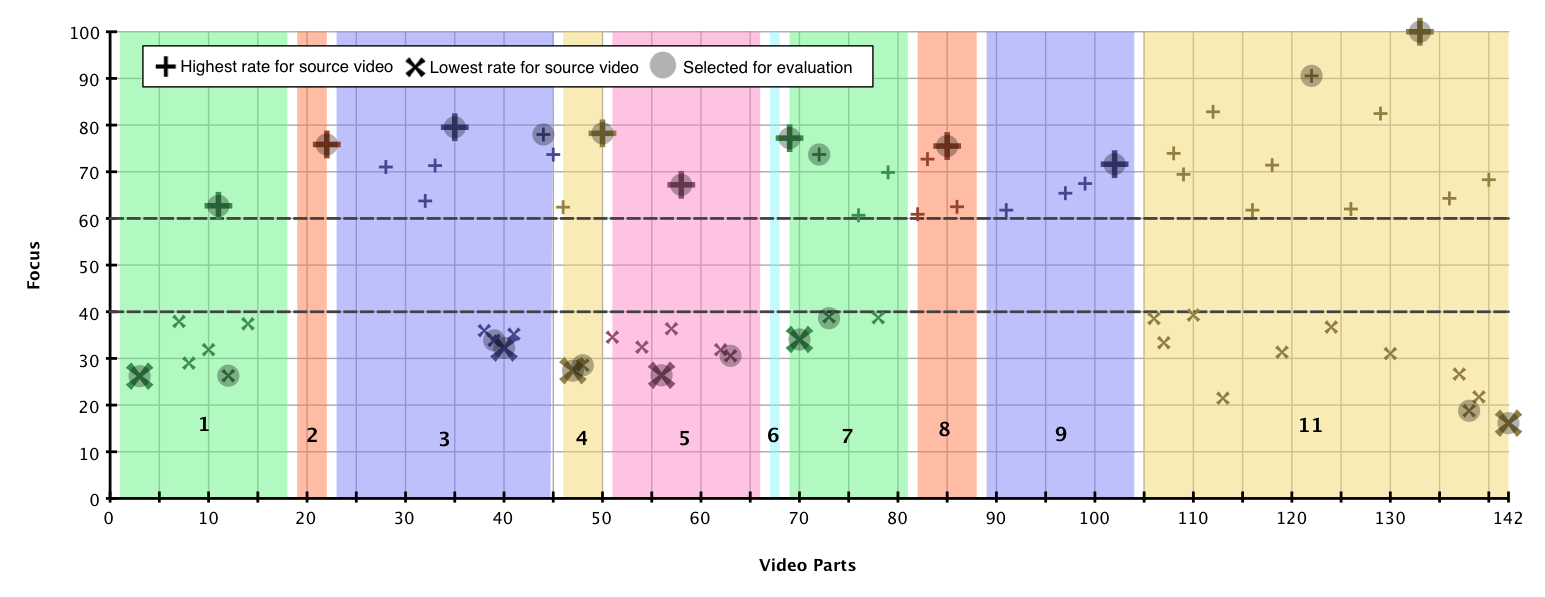
\includegraphics[width=1\textwidth]{img/focus_selection}
  \caption{Video parts considered for filtering based on their focus ratios}
  \label{fig:focus_selection}
\end{figure}

% subsection attention_based_filtering (end)

% subsection reconfiguration (end)

\subsection{Evaluating Focus} % (fold)
\label{sub:evaluating_focus}

By capturing the amount of focus time, we receive measures for user attention. We hypothesise that these measures for attention help point to patterns in user preference. If the two dimensions turn out to be linked, it makes sense to base segmentation (and subsequent reconfiguration) of potentially interesting parts of video on the focus data captured in our parallel play interface.

To see how focus measures relate to user preference, we compare video parts which have received low focus rates to those who received relatively high rates. We construct three types of videos from our data set of video parts based on their weighted focus:
\begin{enumerate}
  \item two complete sets of \emph{parallel play sequence pairs}, one consisting of two sequences of 6 parts from the \emph{best} set, the other consisting of two sequence of 6 from the worst set. For both sets, video parts with the highest (and lowest respectively) focus rates per source video are selected to encourage variety across sources in the reconfiguration.
  \item four \emph{sequences of 6 video parts}, two consisting of the video parts with the highest (lowest) focus rate per source video, two consisting of the 6 video parts with highest (lowest) focus rate that were not yet selected for the parallel play sequences.
  \item twelve \emph{single 10-second video parts}, forming 6 pairs of corresponding video parts with minimum and maximum focus rate for their mutual source video.
\end{enumerate}

Subjects in the evaluation experiment were presented with pairs of content of the three different types described above, one video from the \emph{best} set, the second video from the \emph{worst} set, without subjects knowing the nature of the videos' content. The positioning left or right on screen was done at random to counter possible effects of bias by the positioning. 

After the presentation of the two videos, subjects were asked to rate what they were shown based on how \emph{informative}, \emph{entertaining} and \emph{interesting} they thought the content was. Subjects were instructed to rate content on a range form 1 being very \{uninformative, unentertaining, uninteresting\}, 3 being neutral, 5 being very \{informative, entertaining, interesting\}. 

Besides this, they were asked to choose which of the two presented videos has their preference. Histograms of the received rating are include per video type for each category of assessment below.

\subsubsection{Parallel Play Interaction}
\paragraph{Ratings}

For each of the three dimensions (indicated by colour) of a user's assessment of a parallel played sequence interaction we have plotted how the frequency of the occurrence of the distinct ratings differs for sequences sourced from the selection of video parts with either high focus rates (the best set) or low focus rates (the worst set).

If our hypotheses on the relation between focus and interest are correct, we would expect higher evaluation ratings for the parts that are sourced from the best set, compared to those from the worst set. On the level of parallel sequence interaction this is the case for both entertainment ratings and interest ratings. On these two dimensions, videos from the worst set are more commonly given low ratings, while videos from the best set are more prominent on the high end of the rating spectrum. This is indicated by greater frequency of high ratings for the best set and greater frequency of low ratings for the worst set.

\begin{figure}[htbp]
  \centering
    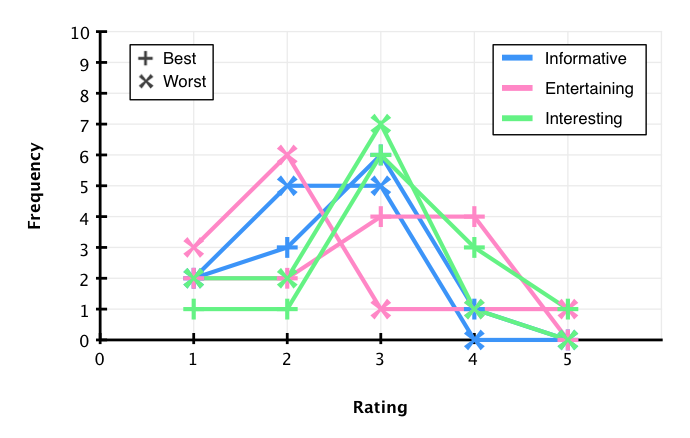
\includegraphics[width=.6\textwidth]{img/evaluation/hist_parallel_key}
  \caption{Histogram of ratings for parallel player sequences}
  \label{fig:evalParallel}
\end{figure}

\paragraph{Preference}
Looking at users' choices for preference does not reveal a very insightful pattern. Although the downward first segment of the line in figure \ref{fig:evalPrefParallel} indicates a collective preference of the interaction featuring content from the best set, the difference is extremely small so not very significant. Because of the small number of subjects it is hard to find telling results. Results that show more extremely difference between the two sets of content are of most relevance.

\begin{figure}[htbp]
  \centering
    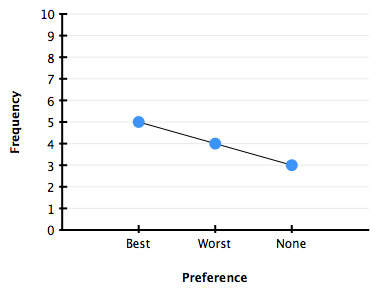
\includegraphics[width=.6\textwidth]{img/evaluation/pref_parallel}
  \caption{Histogram of preferences for parallel sequences}
  \label{fig:evalPrefParallel}
\end{figure}

\subsubsection{Sequences}
\paragraph{Ratings} Of the two sequences we evaluated, the second shows the most indicative configuration of ratings for the dimension of interest. Although not very accentuated we see the same pattern of best set content receiving more high-end ratings and worst set content receiving more low end ratings, with their lines cutting in the middle. 

\begin{figure}
  \centering
  \begin{subfigure}[b]{.5\textwidth}
    \centering
      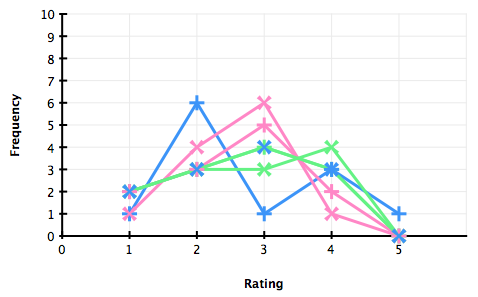
\includegraphics[width=\textwidth]{img/evaluation/hist_seq1}
    \caption{Sequence 1}
    \label{fig:evalSeq1}
  \end{subfigure}%
  ~
    %add desired spacing between images, e. g. ~, \quad, \qquad etc. 
    %(or a blank line to force the subfigure onto a new line)
  \begin{subfigure}[b]{.5\textwidth}
    \centering
      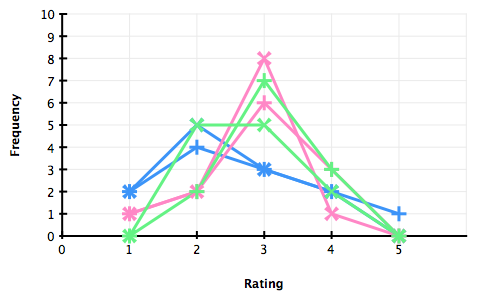
\includegraphics[width=\textwidth]{img/evaluation/hist_seq2}
    \caption{Sequence 2}
    \label{fig:evalSeq2}
  \end{subfigure}
  \caption{Histogram of ratings for two evaluated sequences}
  \label{fig:evalSeqs}
\end{figure}

\paragraph{Preference}

The leaning to `good' content for the second pair of sequences is more clearly accentuated by the choices of preference. Figure \ref{fig:evalSeqsPref} points to a larger difference between the number of people choosing the different sets in favour of the content with high focus rates. 

\begin{figure}[htbp]
  \centering
    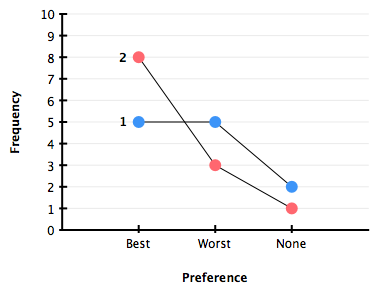
\includegraphics[width=.6\textwidth]{img/evaluation/pref_seqs_all}
  \caption{Histogram of preferences for one minute sequences}
  \label{fig:evalSeqsPref}
\end{figure}

\subsubsection{Video Parts}
\paragraph{Ratings}

Looking at the ratings of the 10-second different videos parts, two videos are most interesting. Video pair 1 and 6 show the most difference in ratings between the two sets of content. Manual inspection of the video parts (originally numbered 11 and 3 in figure \ref{fig:videoparts_focus} for pair 1 and 133 and 142 for pair 6) reveal that both video pairs consist of two pieces of content with a significant difference in activity. Because of the unedited nature of the content used for the experiment, the scene settings are mostly the same. Yet in one of videos (pair 1) originating from the set with high focus ratios, a carriage transporting her majesty Queen Elizabeth passes by in full view and in pair 6 the video from this set shows a zoomed-in shot of a particular boat. The alternative video parts (from the set with low focus ratios) respectively show a couple of horses together with a handful of union jacks and a zoomed out pan-shot capturing many people filming and photographing the Jubilee's boat parade on the river Thames. Video parts in pair three have a similar nature to those in pair 1, but do not show similar patterns in evaluations. The content in the other pairs differs hardly.

\begin{figure}
  \centering
  \begin{subfigure}[b]{.32\textwidth}
    \centering
      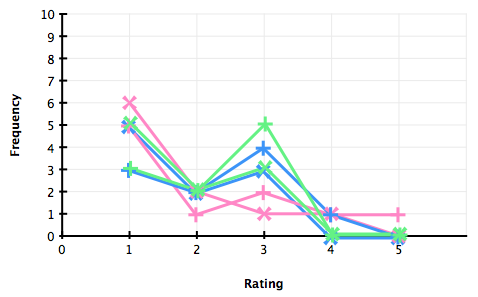
\includegraphics[width=\textwidth]{img/evaluation/hist_video1}
    \caption{Video part pair 1}
    \label{fig:evalVideo1}
  \end{subfigure}%
  ~
    %add desired spacing between images, e. g. ~, \quad, \qquad etc. 
    %(or a blank line to force the subfigure onto a new line)
  \begin{subfigure}[b]{.32\textwidth}
    \centering
      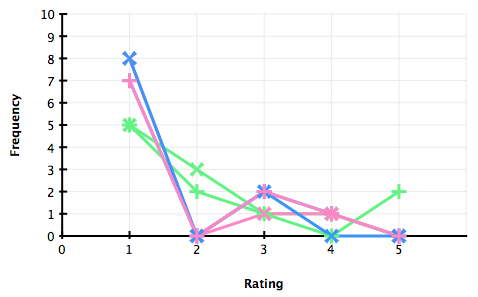
\includegraphics[width=\textwidth]{img/evaluation/hist_video2}
    \caption{Video part pair 2}
    \label{fig:evalVideo2}
  \end{subfigure}
  ~
    %add desired spacing between images, e. g. ~, \quad, \qquad etc. 
    %(or a blank line to force the subfigure onto a new line)
  \begin{subfigure}[b]{.32\textwidth}
    \centering
      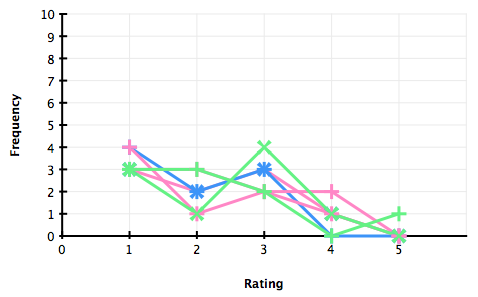
\includegraphics[width=\textwidth]{img/evaluation/hist_video3}
    \caption{Video part pair 3}
    \label{fig:evalVideo3}
  \end{subfigure}
  
  \centering
  \begin{subfigure}[b]{.32\textwidth}
    \centering
      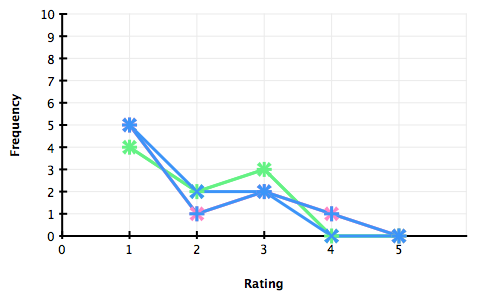
\includegraphics[width=\textwidth]{img/evaluation/hist_video4}
    \caption{Video part pair 4}
    \label{fig:evalVideo4}
  \end{subfigure}%
  ~
    %add desired spacing between images, e. g. ~, \quad, \qquad etc. 
    %(or a blank line to force the subfigure onto a new line)
  \begin{subfigure}[b]{.32\textwidth}
    \centering
      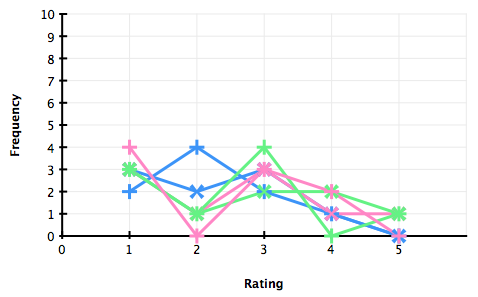
\includegraphics[width=\textwidth]{img/evaluation/hist_video5}
    \caption{Video part pair 5}
    \label{fig:evalVideo5}
  \end{subfigure}
  ~
    %add desired spacing between images, e. g. ~, \quad, \qquad etc. 
    %(or a blank line to force the subfigure onto a new line)
  \begin{subfigure}[b]{.32\textwidth}
    \centering
      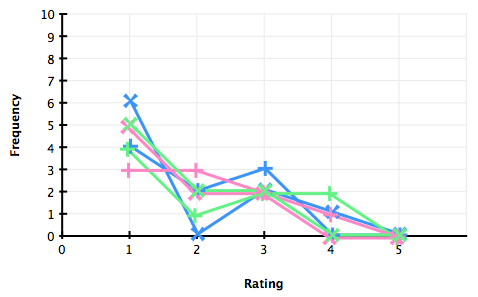
\includegraphics[width=\textwidth]{img/evaluation/hist_video6}
    \caption{Video part pair 6}
    \label{fig:evalVideo6}
  \end{subfigure}

  \caption{Histograms of ratings for six 10-second video parts}
  \label{fig:evalVideos}
\end{figure}

\paragraph{Preference}

The plot of preference frequencies in figure \ref{fig:evalVideosPref} shows an almost unanimous choice for the parts from the best set for pairs 1 and 6. This is a nice result, as it indicates that the distinction by our attentional filtering mechanism corresponds to evaluation of preference for two pair that show a significant difference in contents. While pair three has a similar difference in content between the two videos, subjects show no collective preference for the video from the best set. Overall best set videos have received 38 preferences, while worst set have been preferred only 22 times (32 times no preference was given). While this doesn't indicate a unanimous agreement, it does show correlation between the distinctions made by the attentional filtering and user evaluation. As can be expected the effects are strongest for video parts that differ in content.

\begin{figure}[htbp]
  \centering
    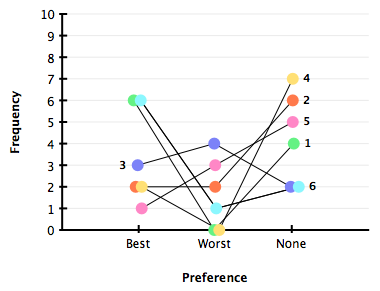
\includegraphics[width=.6\textwidth]{img/evaluation/pref_videos_all}
  \caption{Histogram of preference for 10-second video parts}
  \label{fig:evalVideosPref}
\end{figure}
 

% subsection evaluating_focus (end)
% section main_experiments (end)

\section{Questionnaire} % (fold)
\label{sec:questionnaire}

In addition to the interactive experiment using the parallel play interface subject were presented with a questionnaire asking them about their use of online video and evaluation of the interface. The questionnaire also gave room to express general comments about the experiment. A copy of the questionnaire as presented to the users is included in appendix A.

\subsection{Questions} % (fold)
\label{sub:questions}

\subsubsection{Online Video Content}
To get a better picture of the subjects who participated in the experiment, they were instructed to rate on a discrete scale from one to five the frequency and aggregate daily duration of their interactions with online video as well as how often they feel the content they view is news-related. Figure \ref{fig:quest_consumption} shows amongst others that a large majority of the subjects is accustomed to watching online video on a daily basis, typically for a durations between 10 and 30 minutes.

\begin{figure}[htbp]
  \centering
    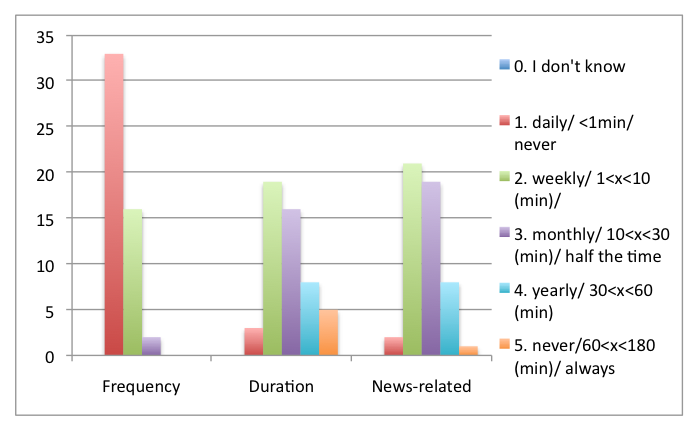
\includegraphics[width=.6\textwidth]{img/evaluation/quest_consumption}
  \caption{Questionnaire Results for questions relating to online video consumption}
  \label{fig:quest_consumption}
\end{figure}

We also asked the users about their own engagement with online video. Figure \ref{fig:quest_own_content} shows that the group of subjects in our experiment include both active and non-active individuals.

\begin{figure}[htbp]
  \centering
    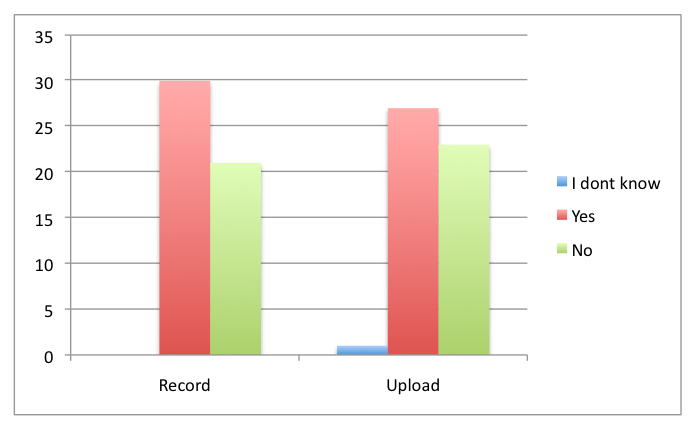
\includegraphics[width=.6\textwidth]{img/evaluation/quest_video}
  \caption{Questionnaire Results for questions relating to user engagement with online video}
  \label{fig:quest_own_content}
\end{figure}
% subsection quesitoins (end)


\subsubsection{The wePorter Interface} 

Subjects seem to slant slightly to a positive evaluation of the interface, but opinions vary. Subjects are also ambivalent about the idea of seeing their own recorded video back in an algorithmic reconfiguration as the one presented in the experiment.

\begin{figure}[htbp]
  \centering
    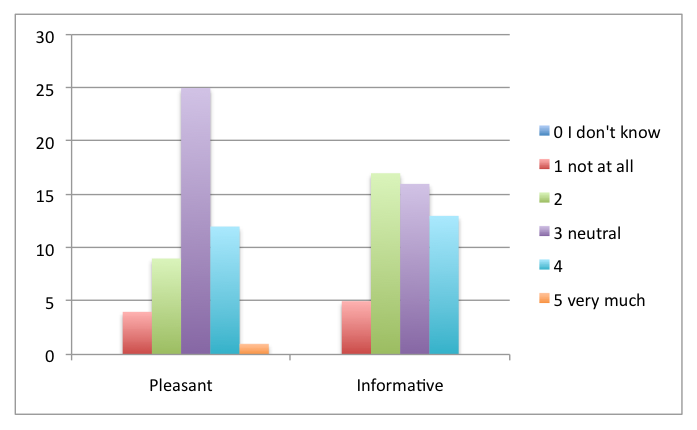
\includegraphics[width=.6\textwidth]{img/evaluation/quest_interaction}
  \caption{Questionnaire Results for questions relating to the wePorter interaction}
  \label{fig:quest_interactions}
\end{figure}

\begin{figure}[htbp]
  \centering
    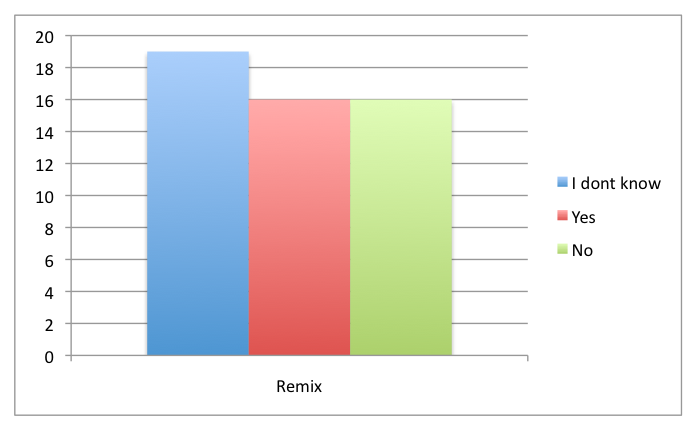
\includegraphics[width=.6\textwidth]{img/evaluation/quest_remix}
  \caption{Questionnaire Results for the question ``Would you like to see your own video content remixed in such a way?''}
  \label{fig:quest_remix}
\end{figure}


\subsection{Feedback from Comments} % (fold)
\label{sub:feedback_from_comments}

\begin{quote}
  ``[...]the technology may [...] have many uses like the crowd sourcing of video editing or the training of AI to mimic human audio visual focus and attention'' - Mia
\end{quote}

As part of the user feedback form, participants were also given the option to leave their comments. Thinking of the potential of the interface, some comments, like the one above, hit the nail right on the head. Others touched upon different aspects of the experiment, the interface and the content of the videos. Overall a number of salient points emerged from the comments:

\begin{itemize}
  \item \textbf{``I would like to see news this way''} - People were positive about the way video was presented in parallel and were enthusiastic about the possibility to interact.
  \item \textbf{``I believe there was a bug''} - A number of people reported difficulties in the playback of videos. Most issues concerned one or more video parts not immediately playing after the preceding one had finished. Besides causing data to be less clean, this caused some users to be confused.
  \item \textbf{``The subject and content of the videos was uninteresting''} - Many people said they were not particularly interested in the topic of the presented videos. This meant that often they weren't drawn strongly to a particular video and did not feel a strong reason to shift focus from one or another.
\end{itemize}

Some participants even offered ideas as to how they saw the project could be extended:

\begin{quote}
  ``Idea is great and project full of potential, in particular for big events which are well covered and allow multi-angle views of an action. It would be interesting to have information about the content producer displayed discretely on the player. That way the audience could vote on the quality of a source, and in time reward the owner for it's content, encouraging him to submit more videos in this system.'' - Marc
\end{quote}

% subsection feedback_from_comments (end)

% section questionnaire (end)

\section{Discussion} % (fold)
\label{sec:discussion}

It is first of all interesting to see which parts of the initial sources videos are picked up by the attention-based filtering mechanism. Manual inspection shows that for source videos that feature intervals of prominent visual activity, parts of this concept can be automatically selected and used in reconfiguration. The low number of interactions per video part definitely contributes to the variation in focus data over time. Increasing the number of interactions per video part will smooth out the data and solidify mountains of attention and valleys of lack of attention.

The initial evaluation performed at multiple levels of reconfigured or deconstructed video, shows that although user evaluations and preferences differ considerably across much of the content, some footage shows signs of correspondence between the time spent focussing by several users on segments of video and the collective evaluation of these parts. Moreover, the global correlation between acquired focus rates and the user preference data acquired in the evaluation experiment, indicate that we are on to something. For six out of the nine pairs of reconfigurations, the `filtered in' piece of content selected for its high focus rates, is evaluated by a majority of the evaluation subjects as most preferential. This is compared to one pair of 10-second video parts where the `filtered out' member received a majority of the preferences.



% section discussion (end)





